\subsection{Conductance-based silicon neuron}

\begin{figure}
    \centering
    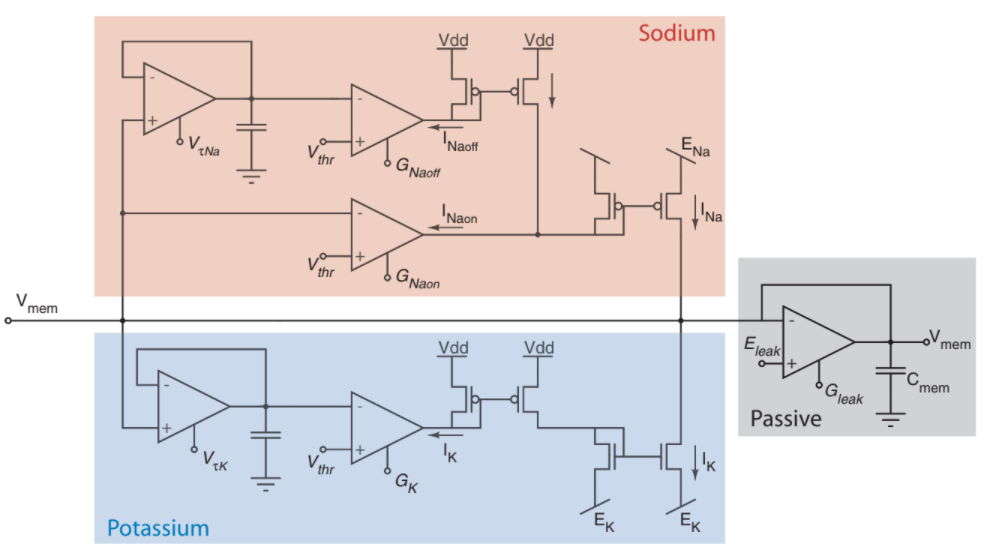
\includegraphics[width=\linewidth]{Figures/conductance_based_neuron.PNG}
    \caption{Conductance-based silicon neuron.}
    \label{fig:conductance_based_neuron}
\end{figure}

In 1991 Misha Mahowald and Rodney Douglas developed a conductance-based silicon neuron that demonstrates remarkably similar properties to those of cortical neurons. The proposed circuit is shown in figure \ref{fig:conductance_based_neuron}. It consists of three part - the passive leak current of the cell membrane, the positive feedback of an action potential that is regulated by sodium in cortical neurons and the negative feedback that is regulated by potassium.\\

\textbf{Passive component}\\

Let's have a look at the circuit's passive component at first. It consists of a follower integrator with output voltage $V_{mem}$ and input voltage $E_{leak}$. The input voltage represents the circuit's resting potential. Remember that the behaviour of the follower integrator can be described by the following equation:

\begin{equation}
    C \frac{d}{dt} V_{out} = I_b tanh (\frac{\kappa (V_{in} - V_{out})}{2 U_T}
\end{equation}

The change in output voltage is dependent on the capacitor's capacitance and the output current of the transconductance amplifier. If $V_{mem} = E_{leak}$, we don't have any output current and consequently the capacitor is neither charged nor discharged. Our output voltage $V_{mem}$ remains unchanged. If $V_{mem}$ becomes larger than $E_{leak}$, a negative current is generated. This current discharges the capacitor and $V_{mem}$ decreases until it equals $E_{leak}$ again. On the other side, when $V_{mem}$ is smaller than $E_{leak}$, we get a positive current that charges the capacitor until $V_{mem} = E_{leak}$. Just looking at our passive component, the membrane voltage always get pulled back to the resting potential $E_{leak}$.\\

\textbf{Sodium positive feedback component}\\

The circuit's positive feedback component consists of another follower integrator and two transconductance amplifiers. Remember from section \ref{sec:transamp_voltage}, that the transconductance amplifier acts as a comparator if it is operated in voltage mode. $V_{out}$ converges towards ground if the input $V_+$ is larger than $V_-$ and towards $V_{dd}$ if $V_- > V_+$. If the circuit's membrane voltage $V_{mem}$ is smaller than $V_{thr}$, we get a large output voltage $V_{out}$ in the lower transconductance amplifier of the sodium component. This voltage is connected to the gate voltage of a pFET current mirror and we consequently have no output current $I_{Na}$. Once our membrane voltage is increased by a positive input signal, $V_{mem}$ eventually becomes larger than $V_{thr}$ and the output voltage $V_{out}$ starts to converge towards zero. This decrease of the gate voltage generates a current flow in the pFET current mirror and we get a positive current $I_{Na}$. This current is equivalent to the current that pushes into our transconductance amplifier as defined by its equation $I_{out} = I_b tanh(\frac{\kappa (V_{thr} - V_{mem})}{2 U_T}$, denoted as $I_{Na,on}$. Note that the source of our current mirror is not set to $V_{dd}$ but to $E_{Na}$. Like this we can ensure that our current is bound by $E_{Na}$. As the connection between $I_{Na}$ and the membrane voltage $V_{mem}$ acts as a capacitor, $V_{mem}$ increases which leads to an even larger current $I_{Na}$. This is the circuit's positive feedback loop. At the same time, $V_{mem}$ is the input voltage of the component's follower integrator. Once $V_{mem}$ starts to increase, the output voltage adapts to the input voltage with a time delay. This delay is dependent on the integrator's capacitance and its bias voltage, denoted as $V_{\tau Na}$ as described in section \ref{sec:follower_integrator}. Once the output voltage becomes larger than the threshold voltage $V_{thr}$ of the top transconductance amplifier, the output voltage converges towards zero and we generate a current flow at our pFET current mirror. This generated current, denoted as $I_{Na,off}$, is connected to the output current of our previous transconductance amplifier. For $I_{Na,off} = I_{Na,on}$, all the current that pushes into our transamp is pulled from $I_{Na,off}$. Consequently, there is no input current into our low current mirror anymore and $I_{Na}$ becomes zero. The top transconductance amplifier is therefore responsible for switching off the positive feedback loop again.\\

\textbf{Potassium negative feedback component}\\

A similar behaviour can be observed in the negative feedback, i.e. the potassium, component of the circuit. The source follower delays the increase of $V_{mem}$ dependent on its bias voltage $V_{\tau_K}$. Once $V_{mem}$ becomes larger than $V_{thr}$ in our transconductance amplifier, our output current $I_K$ is copied by two current mirrors. The resulting current is also connected to the membrane voltage. As it pulls away from the connecting node, an increase of $I_K$ decreases $V_{mem}$. You might wonder why we are using two current mirrors. First of all, we have to ensure that our current flows in the right direction to decrease the membrane voltage. Additionally, the nFET current mirror is not set to ground but to $E_K$. Similar to the positive feedback component, this ensure that $I_K$ is bound by $E_K$.\\

The problem of the proposed circuit is that its behaviour is dependent on a large number of transistors. As introduced in section \ref{sec:device_mismatch}, the expected behaviour of individual transistors can vary up to 20\% due to variations in their fabrication. For a large number of transistors, it becomes impossible to tune all involved variables of the circuit to get the required functionality. We therefore aim to keep our ciruits as minimal as possible.